\documentclass{beamer}
\usepackage[english, russian]{babel}
\usepackage[T2A]{fontenc}
\usepackage[utf8]{inputenc}
\usepackage{indentfirst}
\usepackage{amsmath, amsfonts, amssymb, amsthm, mathtools}
\usepackage[export]{adjustbox}
\usepackage{graphicx} 
\graphicspath{ {./images/} }

\usepackage{subcaption}
\usepackage{verbatim}

\usepackage{minted}{\setlength{\parskip}{0pt}}

\usepackage{hyperref}

\hypersetup{
    colorlinks=true,
    linkcolor=blue,
    filecolor=magenta,      
    urlcolor=black,
    pdftitle={Overleaf Example},
    pdfpagemode=FullScreen,
    }


\title{Отчет по лабораторной работе № 8. \\ Настройка SMTP-сервера}
\author{Данила Стариков \\ НПИбд-02-22}
\date{2024}

\begin{document}

\maketitle
\newpage

\tableofcontents

\newpage
\section{Цель работы}
Приобретение практических навыков по установке и конфигурированию SMTP-сервера.

\newpage
\section{Выполнение работы}

\subsection{Установка Postfix}
\begin{enumerate}
\item На виртуальной машине \texttt{server} вошли под пользователем и открыли терминал. Перешли в режим суперпользователя:
  \begin{minted}{bash}
    sudo -i
  \end{minted}

\item Установили необходимые для работы пакеты:
  \begin{minted}{bash}
    dnf -y install postfix
    dnf -y install s-nail
  \end{minted}

\item Сконфигурировали межсетевой экран, разрешив работать службе протокола SMTP (Рис. \ref{01}):
  \begin{minted}{bash}
    firewall-cmd --add-service=smtp
    firewall-cmd --add-service=smtp --permanent
    firewall-cmd --list-services
  \end{minted}

\begin{center}
    \centering
    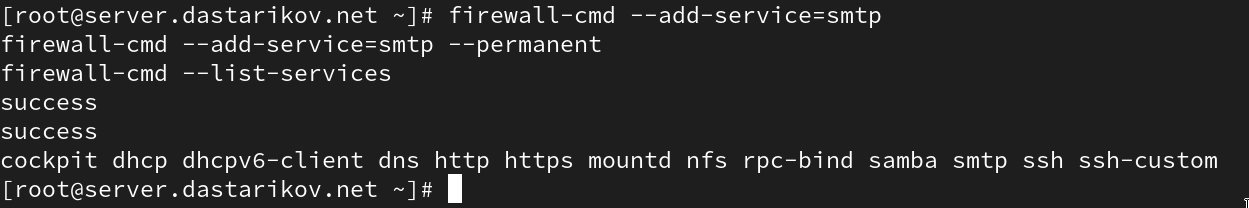
\includegraphics[width=\textwidth]{../images/image01.png}
    \captionof{figure}{Конфигурирование межсетевого экрана.}
    \label{01}
\end{center}

\item Восстановили контекст безопасности в SELinux (Рис. \ref{02}):
  \begin{minted}{bash}
    restorecon -vR /etc
  \end{minted}

\begin{center}
    \centering
    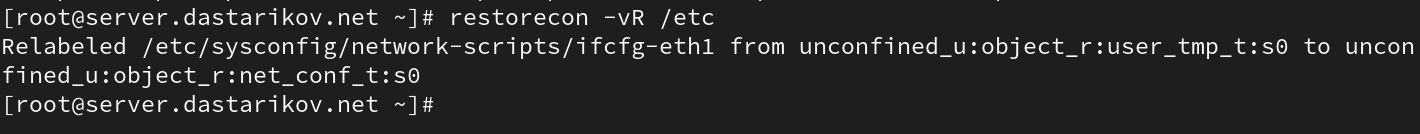
\includegraphics[width=\textwidth]{../images/image02.png}
    \captionof{figure}{Восстановление контекста безопасности SELinux.}
    \label{02}
\end{center}

\item Запустили Postfix (Рис. \ref{06}):
  \begin{minted}{bash}
    systemctl enable postfix
    systemctl start postfix
  \end{minted}
\begin{center}
    \centering
    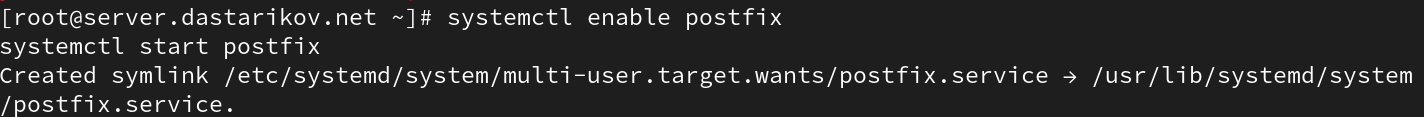
\includegraphics[width=\textwidth]{../images/image06.png}
    \captionof{figure}{Запуск службы Postfix.}
    \label{06}
\end{center}

\end{enumerate}

\subsection{Изменение параметров Postfix с помощью postconf}
Первоначальную настройку Postfix осуществили, используя \texttt{postconf}.

\begin{enumerate}
\item Для просмотра списка текущих настроек Postfix ввели:
  \begin{minted}{bash}
    postconf
  \end{minted}
\item Посмотрели текущее значение параметра \texttt{myorigin} (Рис. \ref{03}):
  \begin{minted}{bash}
    postconf myorigin
  \end{minted}
\item Посмотрели текущее значение параметра \texttt{mydomain} (Рис. \ref{03}):
  \begin{minted}{bash}
    postconf mydomain
  \end{minted}

\begin{center}
    \centering
    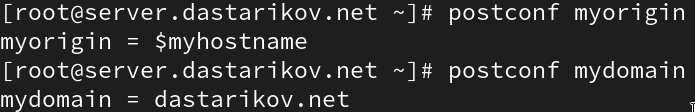
\includegraphics[width=\textwidth]{../images/image03.png}
    \captionof{figure}{Просмотр текущих настроек Postfix.}
    \label{03}
\end{center}

\item Заменили значение параметра \texttt{myorigin} на значение параметра \texttt{mydomain} (Рис. \ref{04}):
  \begin{minted}{bash}
    postconf -e 'myorigin = $mydomain'
  \end{minted}
\item Повторите команду
  \begin{minted}{bash}
    postconf myorigin
  \end{minted}

\begin{center}
    \centering
    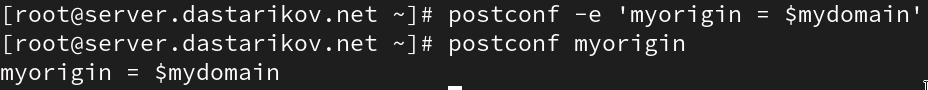
\includegraphics[width=\textwidth]{../images/image04.png}
    \captionof{figure}{Замена значений параметров Postfix.}
    \label{04}
\end{center}

% Убедитесь, что замена параметра была произведена.
\item Проверили корректность содержания конфигурационного файла \texttt{main.cf} (Рис. \ref{05}):
  \begin{minted}{bash}
    postfix check
  \end{minted}
\begin{center}
    \centering
    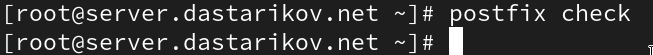
\includegraphics[width=\textwidth]{../images/image05.png}
    \captionof{figure}{Проверка корректности содержания конфигурационного файла \texttt{main.cf}.}
    \label{05}
\end{center}

\item Перезагрузили конфигурационные файлы Postfix (Рис. \ref{07}):
  \begin{minted}{bash}
    systemctl reload postfix
  \end{minted}
\begin{center}
    \centering
    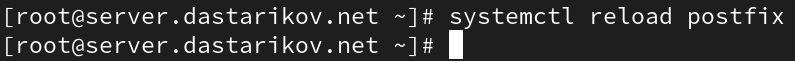
\includegraphics[width=\textwidth]{../images/image07.png}
    \captionof{figure}{Перезагрузка службы Postfix.}
    \label{07}
\end{center}

\item Просмотрели все параметры с значением, отличным от значения по умолчанию (Рис. \ref{08}):
  \begin{minted}{bash}
    postconf -n
  \end{minted}
\begin{center}
    \centering
    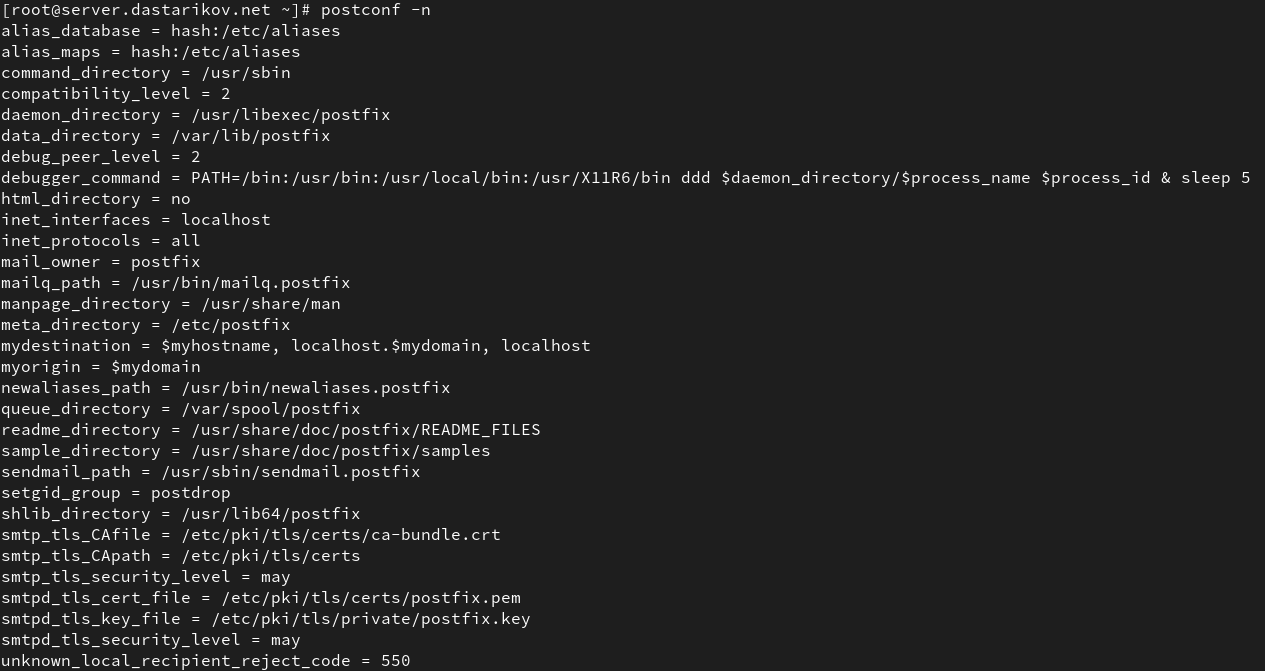
\includegraphics[width=\textwidth]{../images/image08.png}
    \captionof{figure}{Просмотр всех параметров Postfix с отличиями от начальных.}
    \label{08}
\end{center}

\item Задали жёстко значение домена:
  \begin{minted}{bash}
    postconf -e 'mydomain = dastarikov.net'
  \end{minted}
\item Отключили IPv6 в списке разрешённых в работе Postfix протоколов и оставили только IPv4 (Рис. \ref{09}):
  \begin{minted}{bash}
    postconf inet_protocols
    postconf -e 'inet_protocols = ipv4'
  \end{minted}
\begin{center}
    \centering
    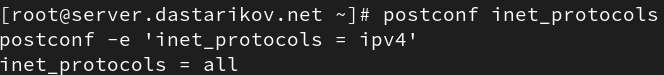
\includegraphics[width=\textwidth]{../images/image09.png}
    \captionof{figure}{Настройка Postfix на работу только с протоколом IPv4.}
    \label{09}
\end{center}

\item Перезагрузили конфигурацию Postfix (Рис. \ref{10}):
  \begin{minted}{bash}
    postfix check
    systemctl reload postfix
  \end{minted}
\begin{center}
    \centering
    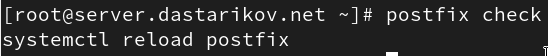
\includegraphics[width=\textwidth]{../images/image10.png}
    \captionof{figure}{Перезагрузка службы Postfix.}
    \label{10}
\end{center}

\end{enumerate}

\subsection{Проверка работы Postfix}
\begin{enumerate}

\item На сервере под учётной записью пользователя отправили себе письмо, используя утилиту \texttt{mail}:
  \begin{minted}{bash}
    echo .| mail -s test1 dastarikov@server.dastarikov.net
  \end{minted}
\item На втором терминале запустили мониторинг работы почтовой службы и посмотрели, что произошло с сообщением (Рис. \ref{11}):
  \begin{minted}{bash}
    tail -f /var/log/maillog
  \end{minted}

\begin{center}
    \centering
    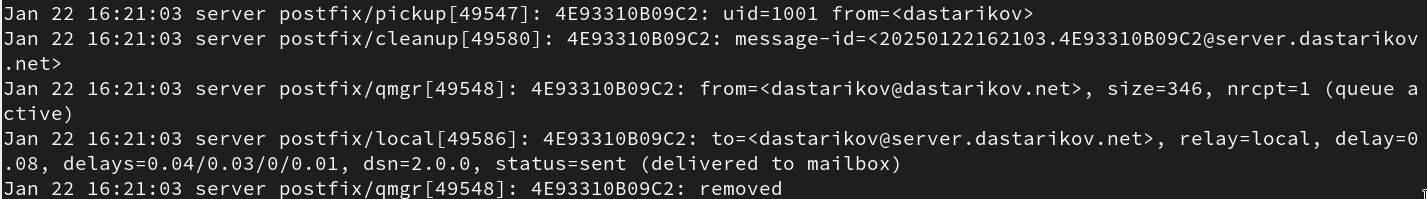
\includegraphics[width=\textwidth]{../images/image11.png}
    \captionof{figure}{Просмотр логов почтовой службы при отправке сообщения.}
    \label{11}
\end{center}

Сообщение доставлено, в логе есть строка "status=sent (delivered to mailbox)".

\item Проверили содержимое каталога \texttt{/var/spool/mail}, где должна храниться информация об отправленном письме (Рис. \ref{12}):
\begin{center}
    \centering
    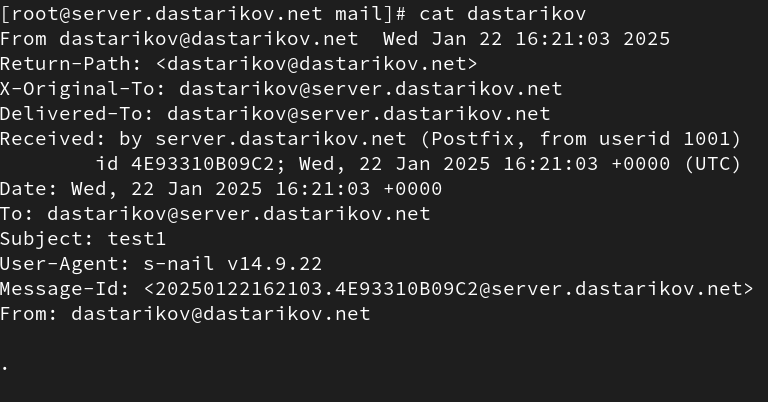
\includegraphics[width=\textwidth]{../images/image12.png}
    \captionof{figure}{Содержимое отправленного сообщения.}
    \label{12}
\end{center}


\item На виртуальной машине \texttt{client} вошли под пользователем и открыли терминал. Перешли в режим суперпользователя:
  \begin{minted}{bash}
    sudo -i
  \end{minted}
\item На клиенте установили необходимые для работы пакеты:
  \begin{minted}{bash}
    dnf -y install postfix
    dnf -y install s-nail
  \end{minted}

\item Отключили IPv6 в списке разрешённых в работе Postfix протоколов и оставьте только IPv4 (Рис. \ref{13}):
  \begin{minted}{bash}
    postconf inet_protocols
    postconf -e 'inet_protocols = ipv4'
  \end{minted}
\begin{center}
    \centering
    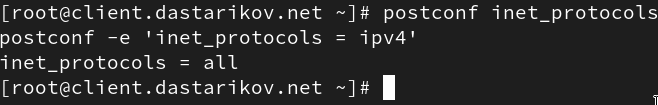
\includegraphics[width=\textwidth]{../images/image13.png}
    \captionof{figure}{Настройка Postfix на работу только с протоколом IPv4 на клиенте.}
    \label{13}
\end{center}

\item На клиенте запустили Postfix (Рис. \ref{14}):
  \begin{minted}{bash}
    systemctl enable postfix
    systemctl start postfix
  \end{minted}
\begin{center}
    \centering
    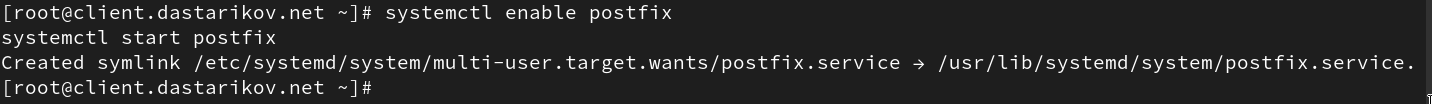
\includegraphics[width=\textwidth]{../images/image14.png}
    \captionof{figure}{Перезапуск службы Postfix.}
    \label{14}
\end{center}

\item На клиенте под учётной записью пользователя аналогичным образом отправили себе второе письмо, используя утилиту \texttt{mail} (Рис. \ref{15}):
\begin{center}
    \centering
    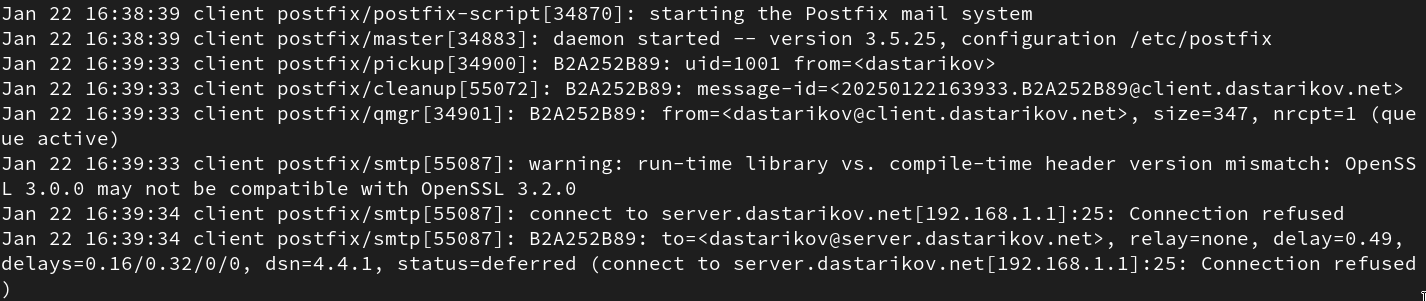
\includegraphics[width=\textwidth]{../images/image15.png}
    \captionof{figure}{Логи при попытке отправить сообщение с клиента.}
    \label{15}
\end{center}
Сообщение не доставлено из-за отказа в доступе к серверу, о чем свидетельствует строка "status=deferred (connect to server <...> Connection refused".

\item На сервере в конфигурации Postfix посмотрели значения параметров сетевых интерфейсов \texttt{inet\_interfaces} и сетевых адресов \texttt{mynetworks} (Рис. \ref{16}):
  \begin{minted}{bash}
    postconf inet_interfaces
    postconf mynetworks
  \end{minted}
\begin{center}
    \centering
    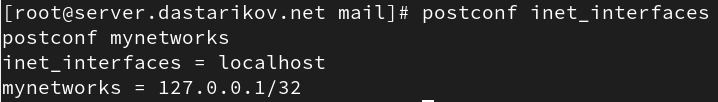
\includegraphics[width=\textwidth]{../images/image16.png}
    \captionof{figure}{Просмотр значений параметров сетевых интерфейсов.}
    \label{16}
\end{center}

\item Разрешили Postfix прослушивать соединения не только с локального узла, но и с других интерфейсов сети (Рис. \ref{17}):
  \begin{minted}{bash}
    postconf -e 'inet_interfaces = all'
  \end{minted}
\item Добавили адрес внутренней сети, разрешив таким образом пересылку сообщений между узлами сети (Рис. \ref{17}):
  \begin{minted}{bash}
    postconf -e 'mynetworks = 127.0.0.0/8, 192.168.0.0/16'
  \end{minted}
\begin{center}
    \centering
    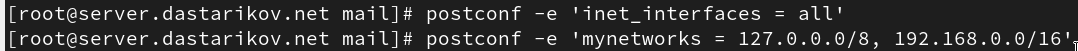
\includegraphics[width=\textwidth]{../images/image17.png}
    \captionof{figure}{Добавление адреса внутренней сети для разрешения пересылки сообщений между узлами сети.}
    \label{17}
\end{center}

\item Перезагрузили конфигурацию Postfix и перезапустили Postfix (Рис. \ref{18}):
  \begin{minted}{bash}
    postfix check
    systemctl reload postfix
    systemctl stop postfix
    systemctl start postfix
  \end{minted}
\begin{center}
    \centering
    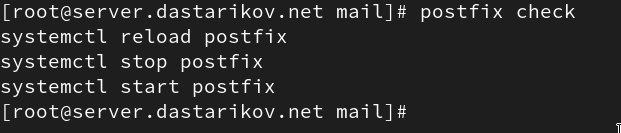
\includegraphics[width=\textwidth]{../images/image18.png}
    \captionof{figure}{Перезагрузка службы Postfix.}
    \label{18}
\end{center}

\item Повторите отправку сообщения с клиента (Рис. \ref{19} и \ref{20}):
\begin{center}
    \centering
    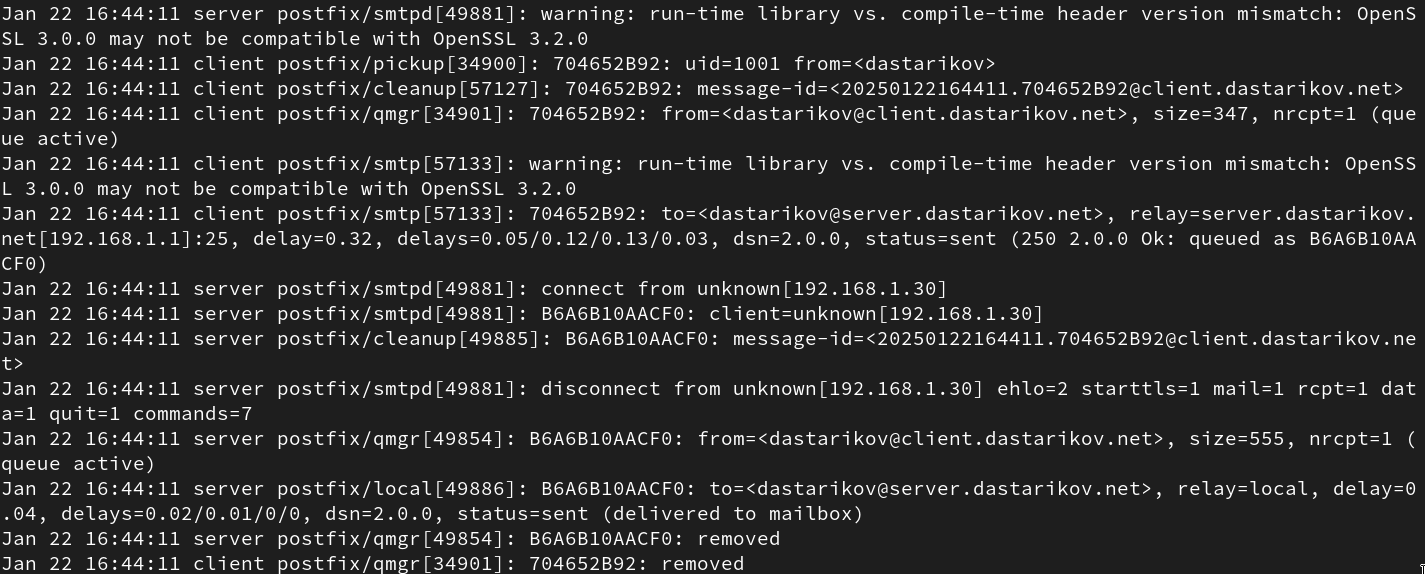
\includegraphics[width=\textwidth]{../images/image19.png}
    \captionof{figure}{Логи при повторной отправке сообщения с клиента.}
    \label{19}
\end{center}
\begin{center}
    \centering
    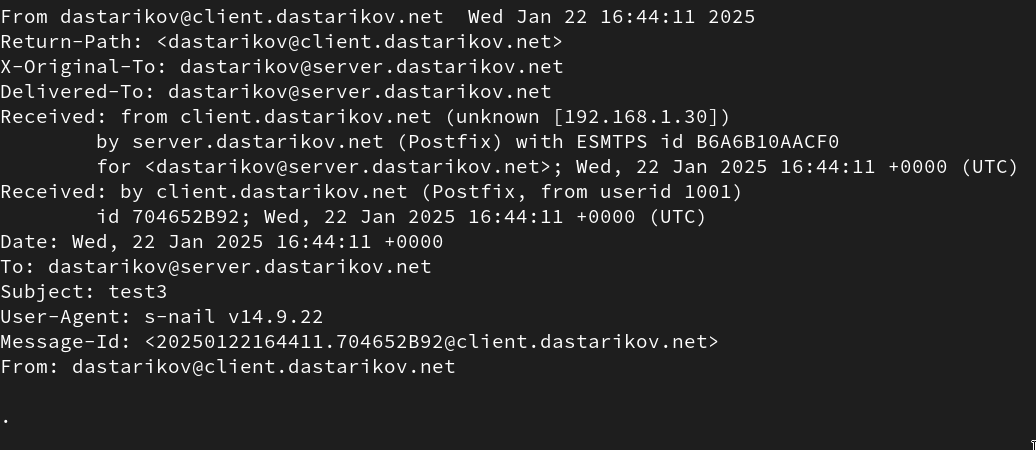
\includegraphics[width=\textwidth]{../images/image20.png}
    \captionof{figure}{Содержимое отправленного  сообщения, хранимое на сервере.}
    \label{20}
\end{center}
\end{enumerate}

\subsection{Конфигурация Postfix для домена}
\begin{enumerate}
\item С клиента отправили письмо на свой доменный адрес:
  \begin{minted}{bash}
    echo .| mail -s test4 dastarikov@dastarikov.net
  \end{minted}

\item Запустили мониторинг работы почтовой службы и посмотрели, что произошло с сообщением (Рис. \ref{21}):
  \begin{minted}{bash}
    tail -f /var/log/maillog
  \end{minted}
\begin{center}
    \centering
    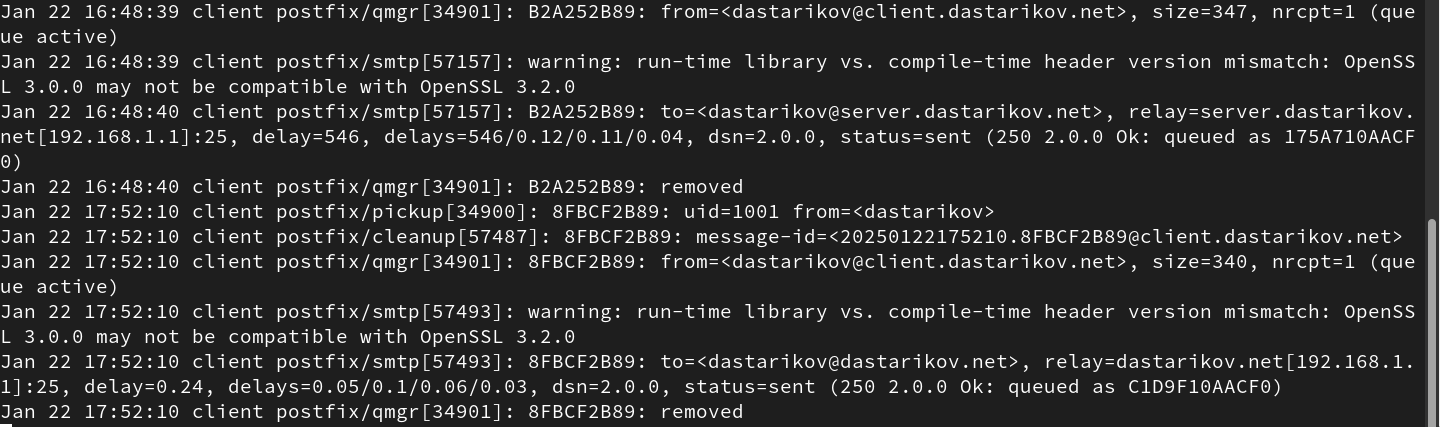
\includegraphics[width=\textwidth]{../images/image21.png}
    \captionof{figure}{Логи при отправке сообщения на доменный адрес.}
    \label{21}
\end{center}


\item Дополнительно посмотрели, какие сообщения ожидают в очереди на отправление (Рис. \ref{22}):
  \begin{minted}{bash}
    postqueue -p
  \end{minted}
\begin{center}
    \centering
    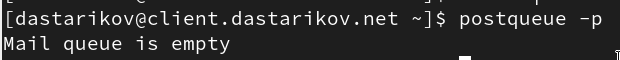
\includegraphics[width=\textwidth]{../images/image22.png}
    \captionof{figure}{Просмотр сообщений в очереди на отправление.}
    \label{22}
\end{center}

\item Для настройки возможности отправки сообщений не на конкретный узел сети, а на доменный адрес прописали MX-запись с указанием имени почтового сервера mail.dastarikov.net в файле прямой DNS-зоны:
  \begin{minted}{bash}
  $TTL 1D
  @       IN SOA    @ server.dastarikov.net. (
                    2020110500             ; serial
                    1D                     ; refresh
                    1H                     ; retry
                    1W                     ; expire
                    3H )                   ; minimum
          NS        @
          A         192.168.1.1
          MX 10     mail.dastarikov.net.
  $ORIGIN dastarikov.net.
  server  A         192.168.1.1
  ns      A         192.168.1.1
  dhcp    A         192.168.1.1
  www     A         192.168.1.1
  mail    A         192.168.1.1
  \end{minted}
и в файле обратной DNS-зоны:
\begin{minted}{bash}
  $TTL 1D
  @       IN SOA    @ server.dastarikov.net. (
                    2020110500             ; serial
                    1D                     ; refresh
                    1H                     ; retry
                    1W                     ; expire
                    3H )                   ; minimum
          NS        @
          A         192.168.1.1
          PTR       server.dastarikov.net.
          MX 10     mail.dastarikov.net.
  $ORIGIN 1.168.192.in-addr.arpa.
  1       PTR       server.dastarikov.net.
  1       PTR       ns.dastarikov.net.
  1       PTR       dhcp.dastarikov.net.
  1       PTR       www.dastarikov.net.
  1       PTR       mail.dastarikov.net.
\end{minted}

\item В конфигурации Postfix добавили домен в список элементов сети, для которых данный сервер является конечной точкой доставки почты (Рис. \ref{25}):
  \begin{minted}{bash}
    postconf -e 'mydestination = $myhostname, localhost.$mydomain, localhost, $mydomain'
  \end{minted}
\item Перезагрузили конфигурацию Postfix (Рис. \ref{25}):
  \begin{minted}{bash}
    postfix check
    systemctl reload postfix
  \end{minted}
\item Восстановили контекст безопасности в SELinux (Рис. \ref{25}):
  \begin{minted}{bash}
    restorecon -vR /etc
    restorecon -vR /var/named
  \end{minted}
\item Перезапустили DNS (Рис. \ref{25}):
  \begin{minted}{bash}
    systemctl restart named
  \end{minted}
\begin{center}
    \centering
    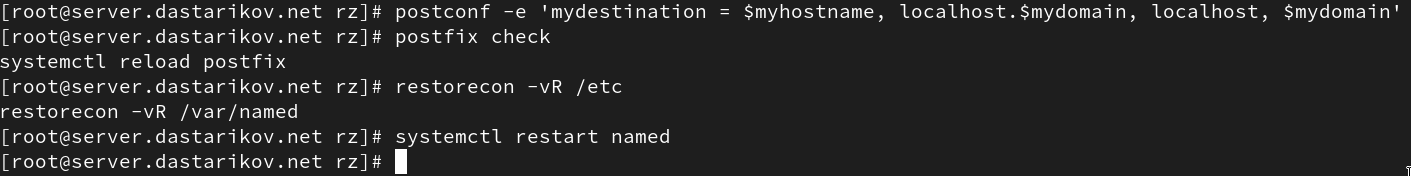
\includegraphics[width=\textwidth]{../images/image25.png}
    \captionof{figure}{Обновление конфигурации Postfix.}
    \label{25}
\end{center}

\item Попробовали отправить сообщения, находящиеся в очереди на отправление:
  \begin{minted}{bash}
    postqueue -f
  \end{minted}
\item Проверили отправку почты с клиента на доменный адрес (Рис. \ref{26} и \ref{27})
\begin{center}
    \centering
    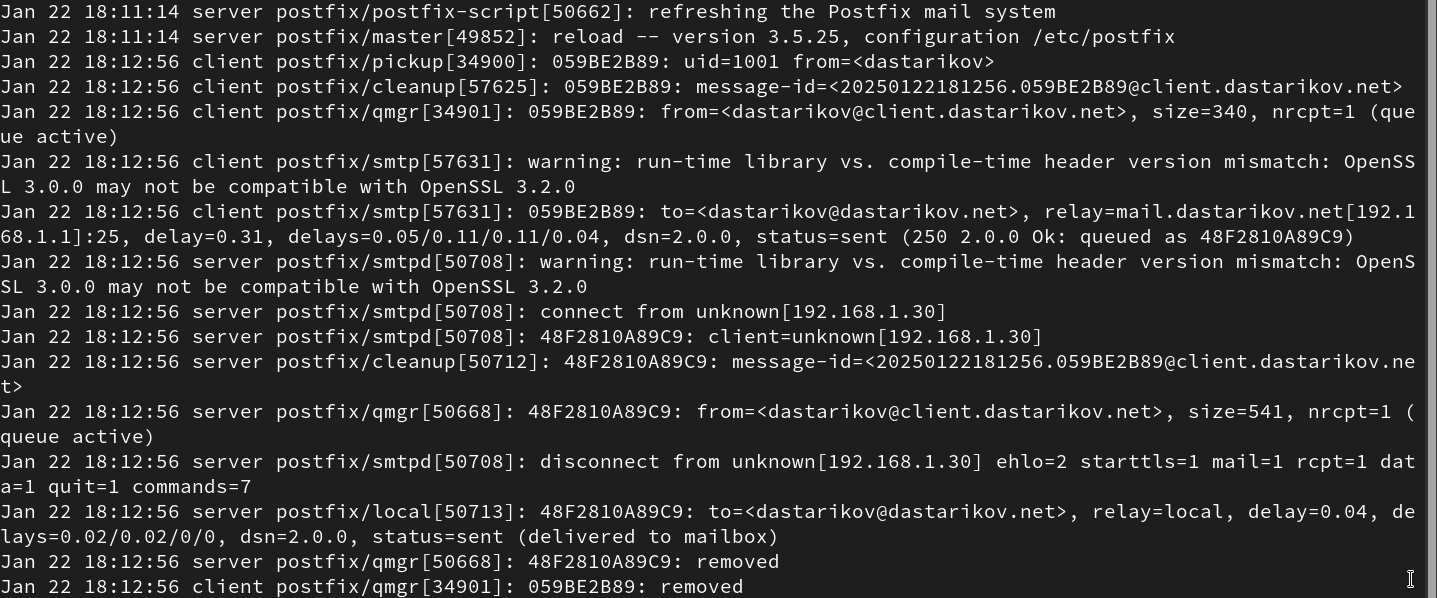
\includegraphics[width=\textwidth]{../images/image26.png}
    \captionof{figure}{Логи при отправке сообщения.}
    \label{26}
\begin{center}
    \centering
    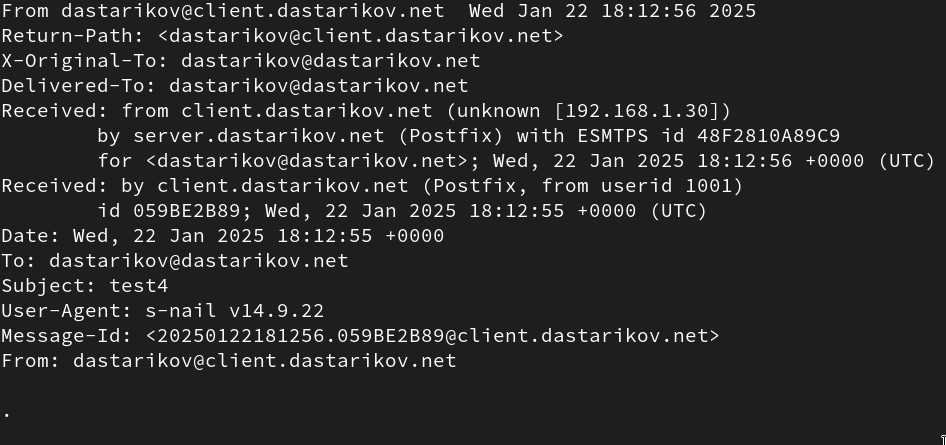
\includegraphics[width=\textwidth]{../images/image27.png}
    \captionof{figure}{Содержание сообщения, хранящееся на сервере.}
    \label{27}
\end{center}

\end{center}

\end{enumerate}
\subsection{Внесение изменений в настройки внутреннего окружения виртуальной машины}
\begin{enumerate}

\item На виртуальной машине \texttt{server} перейдите в каталог для внесения изменений в настройки внутреннего окружения
\texttt{/vagrant/provision/server/}.
\item Заменили конфигурационные файлы DNS-сервера (Рис. \ref{28}):
  \begin{minted}{bash}
    cd /vagrant/provision/server/dns/var/named
    cp -R /var/named/* /vagrant/provision/server/dns/var/named
  \end{minted}
\begin{center}
    \centering
    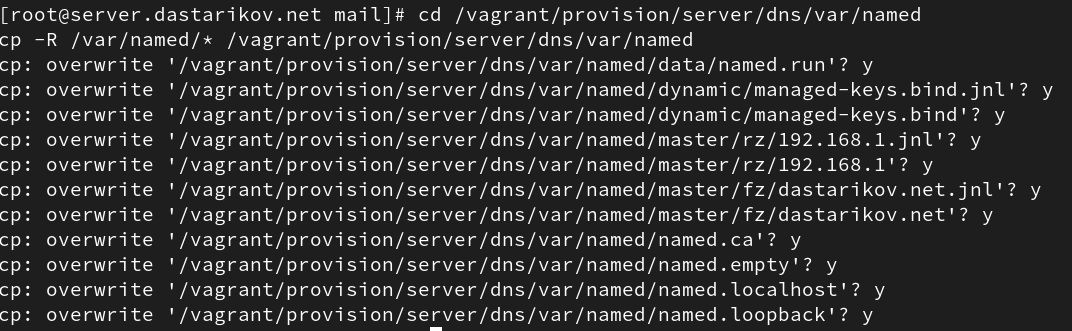
\includegraphics[width=\textwidth]{../images/image28.png}
    \captionof{figure}{Создание каталога для настроек внутреннего окружения.}
    \label{28}
\end{center}

\item В каталоге \texttt{/vagrant/provision/server} создали исполняемый файл \texttt{mail.sh}:
  \begin{minted}{bash}
    cd /vagrant/provision/server
    touch mail.sh
    chmod +x mail.sh
  \end{minted}
Открыв его на редактирование, прописали в нём следующий скрипт:
\begin{minted}{bash}
  #!/bin/bash
  echo "Provisioning script $0"

  echo "Install needed packages"
  dnf -y install postfix
  dnf -y install s-nail
  echo "Copy configuration files"
  #cp -R /vagrant/provision/server/mail/etc/* /etc
  echo "Configure firewall"
  firewall-cmd --add-service=smtp --permanent
  firewall-cmd --reload
  restorecon -vR /etc
  echo "Start postfix service"
  systemctl enable postfix
  systemctl start postfix
  echo "Configure postfix"
  postconf -e 'mydomain = dastarikov.net'
  postconf -e 'myorigin = $mydomain'
  postconf -e 'inet_protocols = ipv4'
  postconf -e 'inet_interfaces = all'
  postconf -e 'mydestination = $myhostname, localhost.$mydomain, localhost, $mydomain'
  postconf -e 'mynetworks = 127.0.0.0/8, 192.168.0.0/16'
  postfix set-permissions
  restorecon -vR /etc
  systemctl stop postfix
  systemctl start postfix
\end{minted}
\item На виртуальной машине \texttt{client} перешли в каталог для внесения изменений в настройки внутреннего окружения \texttt{/vagrant/provision/client/}:
  \begin{minted}{bash}
    cd /vagrant/provision/client
  \end{minted}
\item В каталоге \texttt{/vagrant/provision/client} создали исполняемый файл \texttt{mail.sh}:
  \begin{minted}{bash}
    touch mail.sh
    chmod +x mail.sh
  \end{minted}
Открыв его на редактирование, прописали в нём следующий скрипт:
\begin{minted}{bash}
  #!/bin/bash
  echo "Provisioning script $0"
  echo "Install needed packages"
  dnf -y install postfix
  dnf -y install s-nail
  echo "Configure postfix"
  postconf -e 'inet_protocols = ipv4'
  echo "Start postfix service"
  systemctl enable postfix
  systemctl start postfix
\end{minted}

\item Для отработки созданного скрипта во время загрузки виртуальной машины \texttt{server} в конфигурационном файле Vagrantfile добавили в разделе конфигурации для сервера:
  \begin{minted}{bash}
    server.vm.provision "server mail",
    type: "shell",
    preserve_order: true,
    path: "provision/server/mail.sh"
  \end{minted}
\item Для отработки созданного скрипта во время загрузки виртуальной машины \texttt{client} в конфигурационном файле Vagrantfile добавили в разделе конфигурации для клиента:
  \begin{minted}{bash}
    client.vm.provision "client mail",
    type: "shell",
    preserve_order: true,
    path: "provision/client/mail.sh"
  \end{minted}
\end{enumerate}

\section{Выводы}
В результате выполнения лабораторной работы приобрели практические навыки по установке и конфигурированию SMTP-сервера.
\end{document}
